\section{Theory}\label{sec:theory}

This section discusses the theory behind the models used in the study, with the first section being general information about the soil and use cases of soil temperature in agriculture.

\subsection{Soil temperature}
\todo{remove, and replace with just the practical application}
The difficult in predicting the soil temperature comes from that the environment is highly variant and radically different from each other. A farmer in Sunndal in Middle-Norway would have to do different considerations than a farmer in Karasjok in Nord-Norge or a farmer in Bergen in Sør-Norge simple due to differn climat and soil profile. There exist methods to help farmers get an local estiamte of current soil state; Methods such as soil texture, soil smell, soil feel, and colour. These methods works to make on-the-spot desition to when plant crops, water the crops, or when to harvest. A better approch is to have a model to predict the upcoming temperatures so farmers have a window of time to prepere for crop harvest or planting. \todo{rewrite so it is more accurate but still general, and change chose of place and method}

An application of the soil temperature is used as a mean of agricultural advise is the study conducted by \acrshort{ac:nibio} where they look at the mean five-day air temperature compaired to the mean five-day soil temperature to asses when it is useful to start sowing the seeds\cite{nordskog_jordtemperatur_2018}. 

A way to messure soil temperature is to insert a rod into the ground and messure, however to messure multiple depths there are usally three ways to do it; one rod to messure all the depths, one rod for each depth, and a hybrid solution of the first and the second. There are two sensors that are being used
\begin{enumerate}
	\item Model 107 Temperature Probe\cite{noauthor_107_nodate}
	\begin{itemize}
		\item Tolerance: $\pm0.2^\circ C$ (over the $0^\circ C$ to $50^\circ C$ range)
		\item Measuring Range: $-50^\circ C$ to $+100^\circ C$
		\item Probe Diameter: 0.76 cm (0.3 in.)
	\end{itemize}
	\item PT500 temperature sensor\cite{kamstrup_dokumentasjon_nodate}
	\begin{itemize}
		\item Measuring Range: They have a broad measuring range, usually from $-50^\circ C$ to $+400^\circ C$
		\item Long-term Stability: PT500 sensors are known for their high long-term stability, making them reliable for continuous use over long periods.
		\item Construction: These sensors are constructed with platinum, which contributes to their precise measurements and robustness.
	\end{itemize}
\end{enumerate}
\todo{Add something here between generic and formula. How messure, Why these depths}
There are a few depths to choose to monitor, on of those ranges are 5 cm to 15 cm range that is the root zone\cite{jones_sb_35_nodate}. The root zone is an range where the roots of plants where the highest density of roots are, and at the end of the root zone researchers can gather information about droughts and snow-melts that are filling up og depleting the root system. 

A simple naive way to predict soil temperature would be to use the equation found by \cite{van_wijk_wr_periodic_1963}
\begin{equation}
	\text{daily soil temperature} \approx \widetilde{T}_{\text{soil,year}} + e^{-z/D}\sin(\omega t - z/D + \phi)
\end{equation}

This analytical formula has its limitations as it does not take into account rain fall, snow melt, freezing, and re-freezing. Further more, the formula does not incorporate the importance of the surface temperature and its inpact on the soil layers over time. An ideal formula would incorporate all of these elements and possibly more, but that would require more computation power than currently available.

An expantion of this soultion was expanded by \cite{roodenburg_estimating_1985} by including the solar movement to predict daily soil temperatures. The sun does heat up the soil differently depending on it angle over horizon and the cloud blocking or not hiding the sun. It is commented by the author of \cite{roodenburg_estimating_1985} that this simple model does not describe the soil temperature the effect of snow cover or precipitations effects.

From current understanding of soil physics a modern model researches in cooperate the saturated hydraulic conductivity and the unfrozen water content to their equations\cite{stuurop_influence_2022}. Some of these formulas contains nested exponentials\cite{stuurop_influence_2022}. This formulation introduces numerical limitations as the estimation at the center of the formula would be amplified as the computation continues. A commonly used approch is \acrfull{ac:fdm} where a differential equation gets decomposed to several equation that gets mapped to a grid with boundry conditions\cite{singh_numerical_2017,rankinen_simple_2004,cleall_analytical_2015}. 

\todo{Discuss the problem with predicting soil temeprature}

\subsection{Linear regression}\label{sec:theory:linreg}
\todo{gi grunnlag til hvorfor denne modelen}
Air temperature has a direct connection to soil temperature as the main source of thermal energy next to solar radiation. A primitiv relation between air temperature and soil temperature at a given depth would be

\begin{equation}
	T_{\text{Soil, n cm}} \approx \beta_{\text{n cm}} T_{\text{Air}} + \vec{varepsilon}
\end{equation}
The $\beta_{\text{n cm}}$ represent the scaling factor for the air-soil relation. The regression model will be for the sake of convenience be expressed as the following expression
\begin{equation}
	\vec{F}(\mathbf{A})\vec{\beta}=\vec{y}+\vec{\varepsilon}
\end{equation}

Where $\vec{F}$ is a vector function with following domain $\vec{F}:\mathbb{R}^{n\times m}\to \mathbb{R}^{n\times p}$ where $m,n,p\in \mathbb{N}$, $\mathbf{A}$ is the data in matrix form with dimensions $\mathbb{R}^{n\times m}$, $\vec{\beta}$ is the regression terms with shape $\mathbb{R}^{p\times 1}$, $\vec{y}$ is the target (TJM10 or TJM20) with shape $\mathbb{R}^{n\times 1}$, and $\vec{\varepsilon}$ is the residual error with the same shape as$\vec{y}$.

This basic model to express the linearity of the components to soil temperature. This will function as the base model for regression models. 

\subsection[Plauborg Regression]{Plauborg linear regression model with Fourier terms}\label{sec:theory:pluborg}
The model developed by \cite{plauborg_simple_2002} was trained in Denmark hand has shown promising results for a Scandinavian model. 

An improvement over an time independent linear regression model would be a time dependent linear regression model that takes not only current time into account of the calculations but also previous measurements. It is current knowledge that soil temperatures depends on previous temperatures and meteorological phenomenons. In the paper \citeauthor{plauborg_simple_2002} \cite{plauborg_simple_2002} extend the features from only air temperature at current time to include also previus days of year and the air temperature from those days as an extention of \cite{roodenburg_estimating_1985}. This means the following F function that \citeauthor{plauborg_simple_2002} used would be 
$$
\vec{F} := [air_t , air_{t-1}, air_{t-2}, air_{t-3}, \sin(\omega t) , \cos(\omega t), \sin(2*\omega t), \cos(2*\omega t)]^T
$$

Where $air_t$ is the air temperature at time $t$ expressed in day of the year (0-365), $\omega$ is the angular frequency in radians per hour or radians per day, depending on the time unit. The sine/cosine elements in the F function represent the variations through the day by fitting $\vec{\beta}$ to the yearly variation. To adapt the authors model to an hourly time unit would be to either
\begin{enumerate}
	\item Extend the F function to include a larger $\omega$ coefficient to reflect hourly oscillations in conjunction with daily fluctuation
	\item Refit the Fourier terms with a larger $\omega$ coefficient to make the oscillations more representative of daily temperature changes.
\end{enumerate}

The larger coefficient could be expressed as $\pi/12$ while the smaller $\omega$ for daily values would be rescaled to $2\pi/365$.

The problem with this approach would be Fourier Sine-Cosine series approximation which would suggest that \citeauthor{plauborg_simple_2002}'s method could be subject to overfitting with addition of more terms on a small dataset. On the other hand it gives us a way to compute the coefficients $\alpha_i$ and $\gamma_i$ for sine and cosine terms respectively, though it would be more numerically stable with a pseudo-inverse computation or a max log likelihood approach. However the python module used in this study utilizes a different algorithm described in this paper \cite{van_benthem_fast_2004} that performs an iterative method of solving $\underset{\beta}{\text{argmin}} \left|X\vec{\beta} - \vec{y}\right|$.

\subsection{\acrfull{ac:lstm} model}\label{sec:theory:lstm}

\begin{figure}[ht]
	\centering
	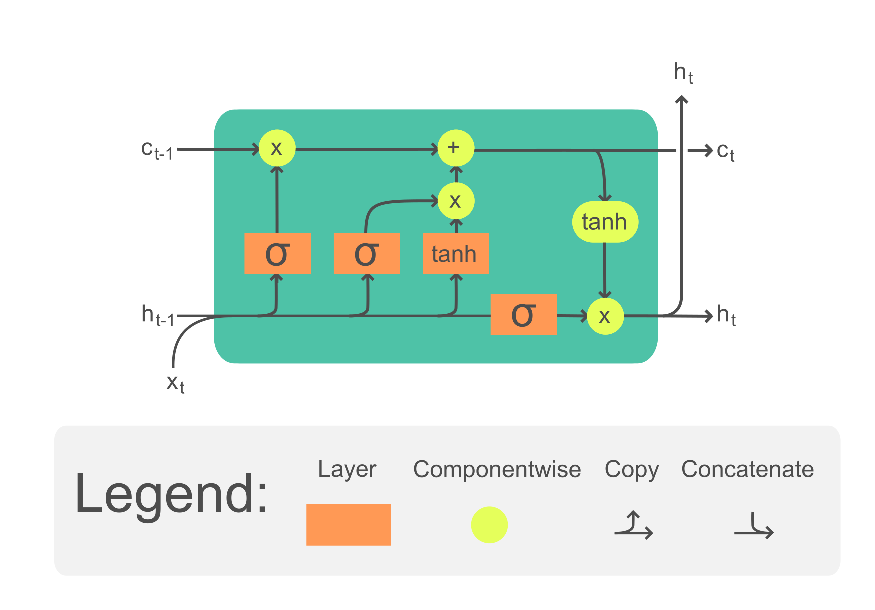
\includegraphics[width=0.7\linewidth]{figures/LSTM_Cell}
	\caption{LSTM cell,  From: \textcite{chevalier_english_2018}}
	\label{fig:lstmcell}
\end{figure}
When modeling soil temperature it is important to know the air temperatures at the previous hours or days to predict the next soil temperature time step, for this a natural selection for a data driven model is a recurrent network. This type of deep learning models makes prediction based on previous time steps in the data, however the longer timespan the model takes into account the less important are the earlier time-steps become according to the model. The LSTM model has been tried in Türkiye \cite{uluocak_daily_2024}, Belgium \cite{elmaz_cnn-lstm_2021}, United States of America \cite{li_modeling_2020} and their findings suggest it is a good model for predicting soil temperature, however it has also been used on a broader dateset spanning 3 continents \cite{li_attention-aware_2022}.

\acrshort{ac:lstm}\cite{hochreiter_long_1997} was developed in the field of Economy to predict the rise and fall of stocks, but has shown to be applicable to other problems that relies on time-series. It has been used to predict soil temperatures\cite{citakoglu_comparison_2017,elmaz_cnn-lstm_2021,feng_estimation_2019,kandasamy_performance_2023,li_attention-aware_2022,li_gans-lstm_2020,li_modeling_2020,wang_modeling_2022,mehdizadeh_modelling_2020} and utelises a method of storing information across the timesteps to preserve information better when predicting, and sending information backwards during training so the earlier weights get adjusted more efficiently. This method is an attempt to solve the problem of the vanishing gradient problem.

The most common problem in training Neural networks is the vanishing gradient problem where updating the first few layers of a large network becomes exponentially more difficult since the adjustments gets smaller and smaller for each layer towards the start rather than the reverse. \gls{gl:lstm} changes this by carrying information from the previous cells forward thereby allowing updating earlier cells with bigger impact than the standard approach\cite{hochreiter_long_1997}. \acrshort{ac:lstm} is part of a family of \gls{gl:rnn}'s that passes information to other cells in the same layer.

LSTMs have proven effective in various tasks outside of economics such as natural language processing, speech recognition, and time series prediction. They provide a powerful mechanism for modeling sequential data while mitigating the vanishing gradient problem commonly encountered in basic RNNs.


\subsection{\acrfull{ac:gru}}

The complexity of soil temperatures and its dependency of previous time-steps make \gls{gl:rnn}'s a natural chose of a deep learning model, but the intricacy of an \acrshort{ac:lstm} makes it difficult to fine tune. An alternative to LSTM is the GRU model\cite{cho_learning_2014} that has fewer parameters to adjust however it has a memory mechanism that allows it to forget and remember information that is passes to other cells in the model. It has been used in Turkey\cite{uluocak_daily_2024}, and China\cite{li_forecasting_2024}

The \acrfull{ac:gru}\cite{cho_learning_2014} was developed in the field of natural language modeling to make translation predictions, however it has been shown that this model is also applicable in other applications than language translation. 

\acrshort{ac:gru} is a simplification of the LSTM cell with fewer total gates, and no output gate. This makes it quicker to train and better for memory deficient computers/servers.

GRU shares similarities with \acrshort{ac:lstm} networks but simplifies the architecture by using two gates: the update gate and the reset gate. These gates allow GRU to selectively retain relevant information from previous time steps while avoiding keeping unnecessary information. The update gate determines how much past information should be passed to the future, while the reset gate controls how much past information to forget. GRU has been effective in various sequence modeling tasks.

\todo{EXPAND, and add formulas}
 
\begin{figure}[H]
	\centering
	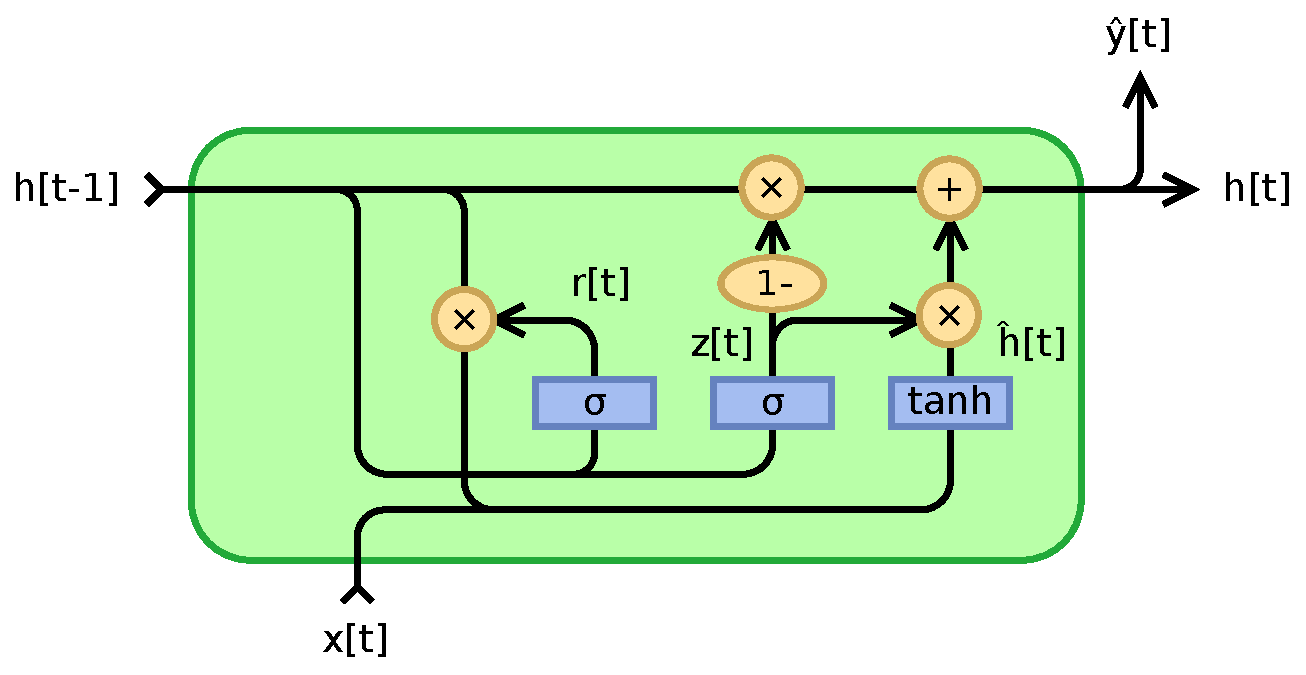
\includegraphics[width = \textwidth]{figures/Gated_Recurrent_Unit_type_2.eps}
	\caption[GRU model sketch]{The GRU model where the memory cell gets more efficiently adjusted by the update gate (z) and appended information via the reset gate (r). From: \cite{jeblad_english_2018}}
\end{figure}

The GRU model offers several advantages over LSTM. It is smaller, converges more efficiently due to the integrated memory and prediction layer, and has fewer gates. These fewer tunable parameters make it faster to train and store the model weights.

\subsection{Bidirectional models}

\begin{figure}
	\centering
	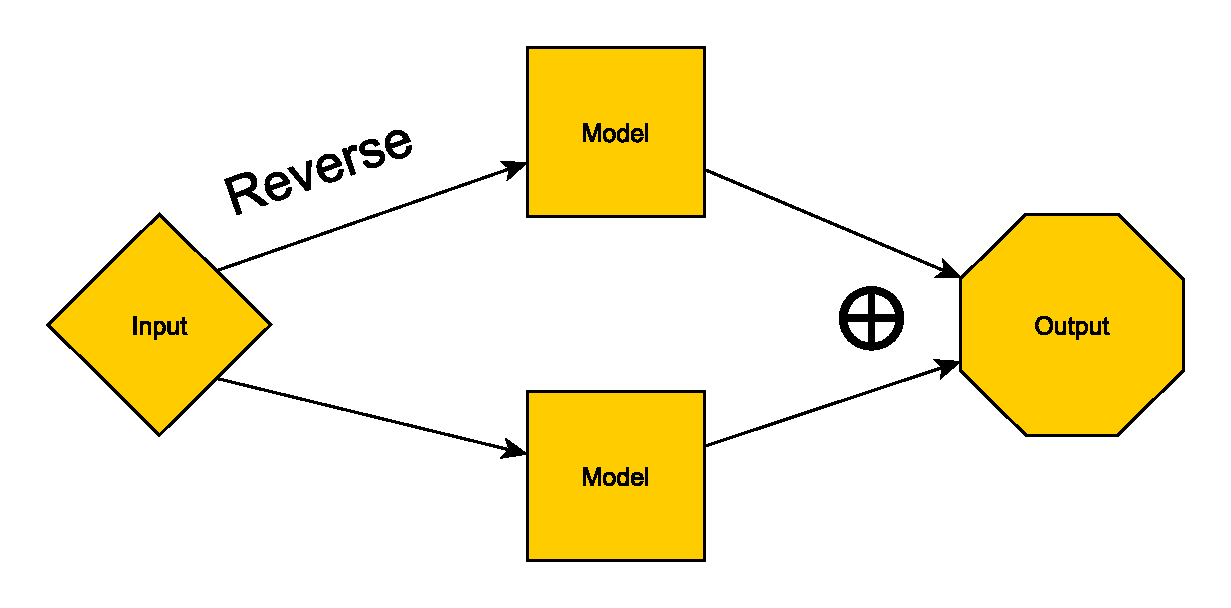
\includegraphics[width=0.8\linewidth]{figures/Bimodel}
	\caption[Bi-directional model diargam]{A diagram of the bidirectional method. The reverse indicates that the input data get reversed before it gets inserted into the model, while the bottom model gets the data. At the end the operator $\bigoplus$ get invoked that combines the output data from both model to a single output. The specifics of this operator can be any operation that combines two vectors to a single vector. In this study the operation is averaging the values.}
	\label{fig:bimodel}
\end{figure}

When making predictions with air temperatures as input, it would be useful to not only make predictions based only on air temperature from $t_0$ to $t_{max}$ as there is information in the reverse time direction, $t_{max}$ to $t_0$. This technique has been applied in other studies with noteworthy performance increase, therefore will be used in this study for both LSTM model and GRU model using the TensorFlow Keras module. 

For the rest of the study a model with the prefix "Bi" indicates that it is a bidirectional model.
